\subsection{Sobre Cross Validation con K-Fold}

Como fue propuesto por la cátedra, para validar que la elección de nuestros parámetros para el sistema lleven luego a una buena generalización al momento de clasificar dígitos, utilizamos la técnica de cross validation con K-Fold.

Brevemente, para el caso de KNN+PCA, por ejemplo, tenemos que elegir entre $(k_i, \alpha_i)$ óptimos, por lo que para cada par se partirá el trainset disponible en $K$ conjuntos para luego hacer $K$ pruebas, donde en cada una de ellas la unión de $K-1$ conjuntos pasan a ser un nuevo trainset y el restante pasa a ser un nuevo testset. Al menos cada conjunto fue un testset después de haber aplicado K-Fold. Luego, promediando alguna métrica de performance entre las $K$ disponibles se puede obtener el valor final para la misma, la cual puede ser comparada después con las generadas por otros pares de parámetros. Los elegidos van a poder ser validados con el testset original.

Las preguntas que se listan a continuación surgieron de pensar las cosas mencionadas en el párrafo anterior y se realizaron pruebas teniendo en cuenta los siguientes atributos:

\begin{itemize}
    \item \textbf{Métrica de performance}: Accuracy, tomando la media.
    \item \textbf{Algoritmo}: KNN+PCA
    \item \textbf{Rango de $K$}: $\{5, 10, 15, 20\}$
    \item \textbf{Rango de $k$}: $\{1\dots53, 2\}$
    \item \textbf{Rango de $\alpha$}: $\{10\dots120, 10\}$
    \item \textbf{Dataset}: Primeros 10000 elementos del dataset original, tomando el $80\%$ como trainset y el restante como testset.
\end{itemize}

\subsubsection{¿Qué valor debería tener $K$?}\label{KFoldValueK}

Elegir los parámetros con validación simple consiste en hacer $n$ corridas de nuestro sistema, donde $n$ es el número de parámetros candidatos que tenemos. Hacerlo con cross validation utilizando K-Fold nos lleva a realizar $n * K$ corridas del sistema, por lo que el tiempo de duración del experimento puede llegar a ser grande. Dependiendo de, entre otras cosas, el tamaño del dataset y la eficiencia general de los algoritmos.

Esto nos llevó a probar inicialmente con una serie de valores fijos para $K$ y una parte del dataset original para ver si, la métrica de performance variaba mucho, e inferir en ese caso si vale el costo temporal o no hacer la validación con valores de $K$ cada vez más altos.

\begin{itemize}
    \item \textbf{Pregunta}: ¿Será apreciable la variación de nuestra métrica de performance si $K$ crece?
    \item \textbf{Hipótesis}: Si: incrementar $K$ permitiría ver como se comporta el sistema con $K$ trainsets distintos, por lo que es factible que mientras más trainsets existan, se van a poder elegir parámetros que generalicen mejor y maximicen la métrica de performance.
\end{itemize}

\subsubsection*{Análisis y resultado}

Para uno de los pares estudiados $(k = 3, \alpha = 40)$

\begin{figure}[H]
    \centering
    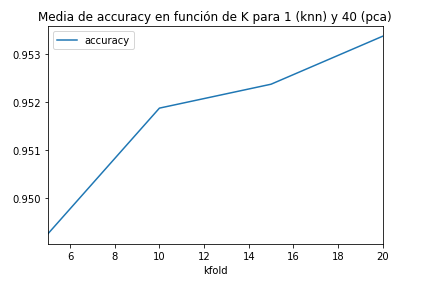
\includegraphics[scale=0.7]{images/KFoldIncreasingK.png}
    \caption{Variación del accuracy en función de $K$ para uno de los pares estudiados.}
    \label{fig:KFoldIncreasingK}
\end{figure}

Como se puede apreciar en la figura \ref{fig:KFoldIncreasingK}, efectivamente, hubo un incremento en el accuracy para $K=5, 10, 15$, pero decreció para $K=20$.

A juzgar por esta prueba, mientras mayor sea $K$, puede presumirse que mayor es el accuracy por lo que parece conveniente, al menos tomar $K=15$.

¿Pero que sucede si tomamos $K$ arbitrariamente grande? Podríamos decir con cierta seguridad que el sistema se encontraría overfitteado, lo que nos llevaría a tener predicciones pobres al validar.

Elegir $K$ arbitrariamente alto tampoco seria productivo.

\subsubsection{¿Qué relación hay entre $K$ y el tamaño del trainset?}\label{KFoldTrainSizeAcc}

Para la siguiente prueba, el trainset definido de 8000 elementos, lo particionamos en cuatro trainsets: el primero de 2000, el segundo de 4000, el tercero de 6000 y el último (el completo) de 8000 elementos.

\begin{itemize}
    \item \textbf{Pregunta}: A mayor tamaño del trainset y de $K$, ¿el accuracy también será mayor?
    \item \textbf{Hipótesis}: Si: de alguna forma será mayor en proporción a la cantidad de elementos que haya en el conjunto de entrenamiento. De esta forma, la mejor elección de nuestros parámetros la vamos a poder realizar con el dataset completo (42000 elementos, 33600 para el trainset) propuesto por la cátedra.
\end{itemize}

\subsubsection*{Análisis y resultado}

La evaluación fue consistente con la hipótesis planteada, observando el par mencionado con anterioridad.

\begin{figure}[H]
    \centering
    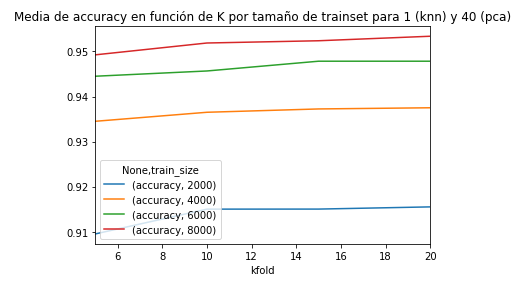
\includegraphics[scale=0.7]{images/KFoldAccTrainSize.png}
    \caption{Accuracy vs $K$: La mayor diferencia parece lograrse no variando $K$, si no variando el tamaño del trainset.}
    \label{fig:KFoldAccTrainSize}
\end{figure}

En la figura \ref{fig:KFoldAccTrainSize} se puede observar, análogamente al caso anterior que para diferentes tamaños de trainset se ven pequeñas mejoras a medida que aumenta el valor de $K$, pero la diferencia notable en el accuracy está precisamente en el tamaño de mencionado conjunto. Aunque también es llamativo ver que la diferencia de la métrica entre el conjunto de 4000 y el de 2000 elementos es mayor a la que hay entre el conjunto de 6000 y 4000 elementos, y a su vez esta es mayor a la diferencia entre el conjunto de 8000 y el de 6000 elementos, lo que nos lleva a pensar que hay un límite para la mejora por el tamaño del trainset y que entrenar nuestro sistema con el dataset completo (42000 * 0.8) puede dejar esta métrica cercano a él.

\subsubsection{¿Conviene utilizar K-Fold? ¿Cuándo no?}

Utilizar K-Fold nos resulta útil para elegir los parámetros con cierta confianza de que no van a haber mayores problemas generalizando a datos desconocidos. A cambio permitimos que la información se reorganice en cada prueba de diferentes maneras. Eso mismo puede ser prohibitivo para modelos en los que haya una componente temporal presente, dado que se pierde el sentido en la información.

Por otra parte, realizar validación simple implica prescindir de una parte de los datos para entrenar, por lo que esta técnica de validación cruzada es particularmente útil en estos casos.

\subsubsection{Finalmente: ¿qué valor debería tener K?}

Vimos en la subsección \ref{KFoldValueK} que podríamos tomar $K=15$, dado que a mayor $K$, mayor accuracy. Pero también comentamos que tomar $K$ arbitrariamente grande puede llegar a ser perjudicial.

En \ref{KFoldTrainSizeAcc} vimos que la mayor confianza se obtiene cuando el trainset tiene un tamaño grande.

De los resultados obtenidos, para la configuración de la prueba mencionada previamente, las que mostraron mayor accuracy fueron:

\begin{table}[h!]
    \begin{center}
        \begin{tabular}{|c|c|c|c|}
        \hline
        \textbf{$K$} & \textbf{$k$} & \textbf{$\alpha$} & \textbf{accuracy medio} \\
        \hline
        5 & 3 & 40 & 0.95\\
        10 & 3 & 40 & 0.9507\\
        15 & 3 & 40 & 0.9516\\
        20 & 5 & 50 & 0.9522\\
        \hline
        \end{tabular}
        \caption{Accuracy medio más alto para distintas configuraciones de K-Fold con un tamaño del trainset de 8000 elementos.}
        \label{kfold_table_1}
    \end{center}
\end{table}

Obteniendo la configuración $(3, 40)$ un accuracy mayor a la que obtuvo el par $(5, 50)$ en el testset final ($0.9645$ vs $0.9625$ respectivamente). Una elección razonable luego, sería tomar $K=15$ para hacer las pruebas. No obstante hay que tener presente que: esto es un ejemplo sobre una porción del dataset original, y el tiempo para calcular las pruebas con ese valor de $K$ puede ser significativo, por lo que finalmente $K=10$ es la elección que tomamos para llevarlas acabo.
